\documentclass[11pt, a4paper]{article}

% --- STANDARD PDFLATEX PACKAGES ---
\usepackage[utf8]{inputenc} % Handle UTF-8 input encoding
\usepackage[T1]{fontenc}    % Use T1 font encoding for better character support
\usepackage{lmodern}        % Use the Latin Modern font family (default for pdflatex)
\usepackage{float}
\usepackage{tabularx}
\usepackage{seqsplit}
\usepackage{listings}
% --- GEOMETRY ---
% Set 1-inch margins
\usepackage[margin=1in]{geometry}

% --- OTHER PACKAGES ---
\usepackage{amsmath, amsfonts} % For math
\usepackage{booktabs} % For tables
\usepackage{hyperref} % For clickable links and references

\hypersetup{
    colorlinks=true,
    linkcolor=blue,
    filecolor=magenta,
    urlcolor=cyan,
}
\usepackage{url} % Better URL formatting
\usepackage{graphicx} % Required for including images (though not used directly here yet)
\lstset{
    basicstyle=\ttfamily\small, % Use typewriter font, slightly smaller
    breaklines=true,          % Enable automatic line breaking
    breakatwhitespace=false,  % Break lines anywhere if needed, not just spaces
    showstringspaces=false,    % Don't put special marks for spaces in strings
    tabsize=2                 % Set tab size (optional)
}
\usepackage{xcolor} % Needed for the postbreak symbol color
% --- DOCUMENT INFORMATION ---
\title{Blockchains and Distributed Ledgers : Smart Contract Programming Coursework Assignment Report}
\author{Royceton Yeoh Tze Jian (s2881515/B299013)} % Replace with your actual student number/name if needed
\date{}

% --- DOCUMENT START ---
\begin{document}

\maketitle
% Content starts immediately after the title

\section{Detailed Contract Design Decisions}
This Vickrey auction contract is designed to facilitate the sale of ERC721 NFTs in a sealed-bid, second-price auction format.

\subsection{Bid Privacy During Bidding Phase}
Bid confidentiality during the active bidding period is maintained using a cryptographic commit-reveal strategy.
\begin{enumerate}
    \item \textbf{Commit Phase:} Bidders do not submit their actual bid value directly. Instead, they compute a hash (commitment) of their bid value combined with a secret nonce (a random string) using the keccak256 algorithm off-chain. This commitment hash is submitted to the contract along with a deposit (an amount of Ether greater than or equal to their intended bid). Because only the hash is stored on-chain during this phase, the actual bid values remain hidden from all participants, preventing information leakage that could influence other bids.
    \item \textbf{Reveal Phase:} After the bidding deadline passes, a second phase begins where bidders reveal their original bid value and the secret nonce they used to create the commitment. The contract recalculates the hash on-chain using the revealed value and nonce. It then compares this recalculated hash with the commitment hash submitted earlier. A bid is only considered valid for winner determination if the revealed information correctly reproduces the original commitment hash. This two-phase process ensures bids are locked in during the first phase and cannot be altered based on subsequently revealed information.
\end{enumerate}

\subsection{Payment to Seller}
To enhance security and robustness, the contract utilises the \textbf{Pull over Push} pattern for transferring the final payment to the seller.
\begin{enumerate}
    \item Upon auction finalisation, the contract identifies the winning bidder and calculates the payment due to the seller. Following Vickrey rules, this payment is the greater of the second-highest valid bid revealed or the seller's predetermined reserve price (or just the reserve price if only one valid bid exists).
    \item Rather than attempting an immediate, direct transfer (push) of Ether to the seller, which could fail or introduce security risks, the contract credits the calculated payment amount to an internal balance associated with the seller's address within the contract storage.
    \item The seller must then actively initiate a separate transaction to withdraw these funds. This withdrawal function first checks the seller's available balance, resets this internal balance to zero (an essential step in the Checks-Effects-Interactions pattern), and proceeds to transfer the Ether to the seller's address.
\end{enumerate}
This pull mechanism makes the payment process more reliable by separating the auction finalisation logic from the complexities and potential failures of external Ether transfers.

\subsection{Prevention of Cheating (Seller/Bidder)}
The contract incorporates several safeguards against malicious behaviour:
\begin{itemize}
    \item \textbf{NFT Escrow:} The seller transfers the NFT into the contract's custody when starting the auction. The contract holds the NFT securely, preventing the seller from transferring it elsewhere during the auction. The NFT is only released to the winner upon successful finalisation or back to the seller if the auction concludes without a valid winning bid.
    \item \textbf{Seller Cannot Bid:} A specific check prevents the address that initiated the auction from participating as a bidder in their own auction. This acts as a direct countermeasure against shill bidding by the seller.
    \item \textbf{Bid Immutability (Commit-Reveal):} The commit-reveal process locks in a bidder's intention during the commit phase. They cannot change their bid amount after the bidding phase ends, nor can they selectively reveal a different bid than the one corresponding to their original commitment hash.
    \item \textbf{Single Bid Per Bidder:} The contract enforces that each bidder address can only submit one commitment per auction. Attempts to submit a second commitment from the same address will be rejected. This prevents strategies involving multiple bids from the same party.
    \item \textbf{Financial Commitment (Deposit Requirement):} Bidders must provide a deposit during the commit phase. During the reveal phase, the contract verifies that the revealed bid amount does not exceed the deposit provided. This ensures that any successfully revealed bid is backed by sufficient funds held in escrow by the contract.
    \item \textbf{Withdrawal Security (Re-entrancy Guard):} The functions handling fund withdrawals are structured to prevent re-entrancy attacks by adhering to the Checks-Effects-Interactions pattern, specifically updating internal balances before initiating external Ether transfers.
\end{itemize}

\subsection{Tie Settlement}
If multiple bidders reveal the identical highest bid amount, the contract resolves the tie based on the time of commitment. The bidder whose commitment transaction was recorded in an earlier block on the blockchain (indicated by a lower block number stored alongside their bid information) is declared the winner. This provides a deterministic and fair tie-breaking rule based on who committed their intention first.

\subsection{Multiple Bids Handling}
The contract design strictly prohibits a single bidder address from submitting more than one bid commitment within the same auction. This restriction is enforced during the commit phase by checking if the bidder already has a non-zero commitment hash stored for that specific auction. If a prior commitment exists, any subsequent commit attempts from that same address for that auction will fail, reverting the transaction.

\subsection{Data Types and Structures}
Appropriate data types and structures are used for clarity, efficiency, and safety:
\begin{itemize}
    \item \textbf{Structs (`Auction`, `Bid`):} Custom structures group related data logically. In this contract's case, all details pertaining to an auction and all details for a specific bid. This improves code readability and organisation.
    \item \textbf{Mappings (`auctions`, `bids`, `pendingWithdrawals`):} Mappings serve as key-value stores, providing efficient (constant-time complexity) lookups. \texttt{auctions} maps IDs to auction data, \texttt{bids} uses a nested structure (auction ID -> bidder address -> bid data) for direct access to any specific bid, and \texttt{pendingWithdrawals} tracks withdrawable balances per address.
    \item \textbf{Numerical Types (`uint256`):} The standard unsigned 256-bit integer is used for monetary values (Ether amounts are handled in Wei), token IDs, timestamps, durations, block numbers, and counters, aligning with EVM practices and providing a large range.
    \item \textbf{Addresses (`address payable`):} Addresses eligible to receive Ether (sellers and bidders) are marked as payable.
    \item \textbf{Hashes (`bytes32`):} The 32-byte type is used for storing commitment hashes, matching the output sise of the keccak256 algorithm.
    \item \textbf{Booleans (`bool`):} Used for simple status flags (e.g., whether an auction is active, finalised, or a bid revealed).
    \item \textbf{Interfaces (`IERC721`):} Using the standard interface type allows the auction contract to interact generically with any compliant ERC721 NFT contract for ownership checks and transfers.
\end{itemize}
These choices reflect standard Solidity practices, aiming for gas efficiency in common operations like data lookups while maintaining type safety and code clarity.

\section{Gas Evaluation}
\subsection{Deployment and Interaction Costs}
Transaction costs (in Gwei) based on observed Sepolia network interactions with a gas price of 1.500000011 Gwei
\begin{itemize}
    \item Contract Deployment: 3739308.02492872 Gwei (Most expensive operation due to storing the contract bytecode on-chain).
    \item \texttt{startAuction}: 295918.501775511 Gwei (High cost due to multiple storage writes for new auction struct and the external NFT \texttt{\detokenize{safeTransferFrom}} call).
    \item \texttt{commitBid}: 149859.00099906 Gwei (Primary cost from writing bidder's commitment and deposit to storage).
    \item \texttt{revealBid}: 168672.001236928 Gwei (Higher cost due to on-chain hash calculation, conditional winner logic, and potential multiple storage updates for auction winner/price fields).
    \item \texttt{finalisedAuction}: 191835.00166257 Gwei (High cost due to storage updates marking auction as finalised and the external NFT \texttt{\detokenize{safeTransferFrom}} call to winner or seller).
    \item \texttt{claimLosingBid}: 70506.000517044 Gwei (Involves reading and updating storage for the specific bid and the bidder's withdrawable balance).
    \item \texttt{withdrawFunds}: 45487.500333575 Gwei (Involves storage update to zero balance and an external call to transfer Ether).
\end{itemize}

\subsection{Fairness}
Discuss gas fairness:
\begin{itemize}
    \item \textbf{Auction Finalisation:} The \texttt{finalisedAuction} function can be called by anyone after the reveal period ends. The caller bears the gas cost for this potentially complex transaction (determining winner, calculating payment, transferring NFT). This could be seen as unfair if one party consistently has to trigger it. However, making it callable by anyone ensures the auction can be finalised even if the seller or winner is unresponsive.
    \item \textbf{Withdrawals:} The pull-pattern shifts the gas cost of receiving funds (\texttt{claimLosingBid} and \texttt{withdrawFunds}) entirely onto the beneficiaries (seller, refunded winner, losing bidders). While this adds steps and costs for users, it prevents burdening other functions with potentially unbounded loops or complex payout logic, which could lead to DoS. It can be argued this is fairer, as each user pays for their own withdrawal transaction.
    \item \textbf{Bidding Costs:} Gas costs for \texttt{commitBid} and \texttt{revealBid} should be relatively consistent for all bidders, promoting fairness during the core auction phases. Small variations might occur based on data sizes (e.g., zero vs non-zero storage writes), but significant systemic unfairness isn't apparent in these functions.
\end{itemize}


\subsection{Cost Efficiency and Fairness Techniques}
\begin{itemize}
    \item \textbf{Pull-over-Push Pattern:} This enhances security and prevents unbounded gas costs in finalisation, shifting withdrawal costs to beneficiaries. This is a deliberate tradeoff favoring security and robustness over minimising transactions for users.
    \item \textbf{Data Structures:} Mappings provide efficient O(1) lookups, minimising gas for reading auction/bid data. Structs keep data organised without significant overhead.
    \item \textbf{Solidity Version:} Using \texttt{pragma solidity \^{}0.8.0;} leverages the built-in overflow/\newline underflow checks, which are generally more gas-efficient than importing and using external SafeMath libraries required in older versions.
    \item \textbf{Minimal Logic:} Functions generally perform only necessary actions. For instance, \texttt{finalisedAuction} doesn't attempt to refund all losers in a loop.
\end{itemize}

\section{Potential Vulnerabilities, Hazards, and Mitigation}
This section details potential security risks and the mechanisms implemented in the contract to mitigate them.

\subsection{Identified Vulnerabilities/Hazards}
Common smart contract vulnerabilities considered during design include:
\begin{itemize}
    \item Re-entrancy attacks on withdrawal functions.
    \item Front-running during commit or reveal phases.
    \item Miner manipulation of timestamps (\texttt{block.timestamp}) affecting deadlines.
    \item Denial-of-Service (DoS) through gas limits or logic errors.
    \item Integer Overflow/Underflow bugs.
    \item Insufficient Access Control or Authorisation issues.
    \item Handling of incorrect or malicious inputs.
\end{itemize}

\subsection{Security Mechanisms and Mitigation}
The contract employs several strategies to address these potential issues:
\begin{itemize}
    \item \textbf{Re-entrancy:} Mitigated primarily using the \textbf{Checks-Effects-Interactions pattern} in functions involving ETH transfer. Specifically, in \texttt{withdrawFunds}, the balance is zeroed (\texttt{pendingWithdrawals[msg.sender] = 0;}) before the external call (\texttt{msg.sender.call\newline\{value: amount\}("")}). Similarly, in \texttt{claimLosingBid}, the deposit is zeroed (\texttt{bid.\newline deposit = 0;}) before updating \texttt{pendingWithdrawals}. The overall \textbf{Pull-over-Push pattern} for all fund retrievals further minimises re-entrancy risks by isolating transfers into separate transactions initiated by the user.
    \item \textbf{Front-Running:} The \textbf{Commit-Reveal Scheme} protects bid values, as only hashes are visible during bidding. The commit transaction itself remains vulnerable to front-running for griefing (forcing a user to recommit) or attempts to claim the bid slot, although the bid value remains secret. Front-running the reveal does not alter the outcome based on bid value, as the bidding phase is closed.
    \item \textbf{Timestamp Dependence:} Deadlines (\texttt{biddingEndTime}, \texttt{revealEndTime}) rely on \newline \texttt{block.timestamp}. While miners have minor control over timestamps, significant manipulation is difficult and costly. Using timestamps for deadlines is standard practice. The durations are set relative to the start time, providing a predictable window. The risk is considered low for typical auction durations.
    \item \textbf{Gas Limit Issues (DoS):} The pull pattern for withdrawals (\texttt{claimLosingBid} and \texttt{withdrawFunds}) avoids loops over arrays of bidders, which could otherwise lead to unbounded gas costs exceeding block limits as the number of bidders grows. This prevents DoS attacks aimed at making payouts impossible. Functions such as \texttt{revealBid} have bounded complexity.
    \item \textbf{Integer Overflow/Underflow:} The contract uses \texttt{pragma solidity \^{}0.8.0;}. Versions 0.8.0 and above include built-in checks for arithmetic overflow and underflow, automatically reverting the transaction if such conditions occur. This eliminates the need for external SafeMath libraries for standard arithmetic operations.
    \item \textbf{Access Control:} Multiple \texttt{require} statements enforce rules: only the NFT owner can start the auction (\texttt{nftContract.ownerOf(\_tokenId) == msg.sender}), sellers cannot bid (\texttt{msg.sender != auction.seller}), bids/reveals must happen within the correct phases, reveals must match commitments (\texttt{bid.commitment == commitment}), winners cannot use \texttt{claimLosingBid} (\texttt{msg.sender != auction.highestBidder}), etc.
    \item \textbf{Incorrect Inputs:} \texttt{require} statements validate critical inputs like positive auction durations, non-zero deposits (\texttt{msg.value > 0}), and non-zero commitments (\texttt{\_commitment != bytes32(0)}).
    \item \textbf{Single Commit Enforcement:} The contract prevents multiple commits per bidder per auction using \texttt{require(bids[\_auctionId][msg.sender].commitment == bytes32(0), ...)}.
    \item \textbf{Deposit Requirement:} The check \texttt{require(bid.deposit >= \_bidAmount)} ensures revealed bids are financially backed, preventing bidders from revealing unaffordable amounts.
\end{itemize}


\section{Tradeoffs and Choices}
Several design decisions involved balancing competing factors like security, user experience, gas efficiency, and fairness.
\begin{itemize}
    \item \textbf{Security vs. User Experience (Pull vs. Push):} The most significant tradeoff is the use of the pull-over-push pattern for all ETH withdrawals (\texttt{withdrawFunds}, \texttt{claimLosingBid}). This pattern significantly enhances security against re-entrancy\newline attacks and potential DoS issues related to failed transfers or gas limits if the contract were to push funds automatically. However, it degrades user experience as it requires beneficiaries (seller, refunded winner, losing bidders) to send 1-2 additional transactions (\texttt{claimLosingBid} if applicable, then \texttt{withdrawFunds}) to retrieve their ETH, incurring extra gas costs and steps. A push pattern would be more convenient but riskier. Security was prioritised here.
    \item \textbf{Fairness vs. Efficiency (Gas Costs):} The pull pattern shifts the gas cost of withdrawals to the users receiving funds. This can be seen as fairer than having the \newline \texttt{finalisedAuction} caller or the contract potentially pay for multiple transfers, but it does impose costs on users. The fact that anyone can call \texttt{finalisedAuction} is efficient in ensuring finalisation but means the caller bears that gas cost, which might not always be the seller or winner. The tie-breaking mechanism using \texttt{commitBlock} is computationally simple and efficient, avoiding potentially more complex or gas-intensive methods, while providing a deterministic outcome.
    \item \textbf{Simplicity vs. Feature Richness:} The contract implements the core Vickrey auction logic with commit-reveal but omits features like auction cancellation, automatic extensions if bids occur near the end, proxy bidding, or more complex dispute resolution. This focus on simplicity reduces the potential attack surface and contract complexity, potentially enhancing security and auditability, at the cost of fewer features.
    \item \textbf{On-chain vs. Off-chain Logic:} All essential logic determining the auction state, validity of bids, winner, and payment amounts is performed on-chain. This ensures transparency and trustlessness, as all participants can verify the auction's execution based on blockchain data. The only off-chain components are the user-side calculation of the commitment hash and the monitoring of auction phases. Relying more heavily on off-chain components could potentially reduce gas costs but would likely compromise transparency or require additional trust assumptions.
\end{itemize}

\section{Analysis of Fellow Student's Contract}
\subsection{Contract Address}
Fellow Student's Sepolia Contract Address: [0xC8269b326055480513cB655a03d22963e4D342f4]

\subsection{Security, Efficiency, Fairness Analysis}
\textbf{Security:}
\begin{itemize}
    \item \textbf{Re-entrancy Protection:} Uses OpenZeppelin's \texttt{\detokenize{ReentrancyGuard}} (\texttt{\detokenize{nonReentrant}} modifier) on key state-changing functions (\texttt{\detokenize{startAuction}}, \texttt{\detokenize{endAuction}}, \texttt{\detokenize{withdraw}}). The \texttt{\detokenize{withdraw}} function also follows Checks-Effects-Interactions by deleting the bid record (\texttt{\detokenize{delete committedBids[_auctionId][msg.sender];}}) before the external ETH transfer (\texttt{\detokenize{msg.sender.safeTransferETH(_collateral);}}). The \texttt{\detokenize{endAuction}} function performs state updates (\texttt{\detokenize{active = false;}}, \texttt{\detokenize{auctionId++;}}, \texttt{committedBids[finishedId]\newline[highestBidder].collateral = difference;}) before external calls.
    \begin{figure}[H]
        \centering
        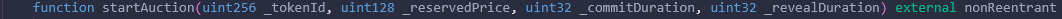
\includegraphics[width=1.0\linewidth]{../Images/startAuction.png}
        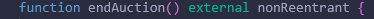
\includegraphics[width=1.0\linewidth]{../Images/endAuction.png}
        
\includegraphics[width=1.0\linewidth]{../Images/withdraw.png}
        \caption{Code Snippet of nonReentrant modifier}
    \end{figure}
    \item \textbf{Overflow/Underflow:} Use of \texttt{\detokenize{pragma solidity ^0.8.19;}} provides automatic protection. Using \texttt{\detokenize{uint128}} for amounts/collateral provides an additional layer against excessively large values.
    \item \textbf{Input Validation:} Strong validation exists in \texttt{\detokenize{startAuction}} (ownership, approval, durations, reserve price). \texttt{\detokenize{commitBid}} checks auction phase, non-zero hash, and commit limit. \texttt{\detokenize{revealBid}} checks phase, committed bid existence, reveal status, hash matching, and deposit coverage (\texttt{\detokenize{if(bid.collateral >= amount){...}}}).
    \begin{figure}[H]
        \centering
        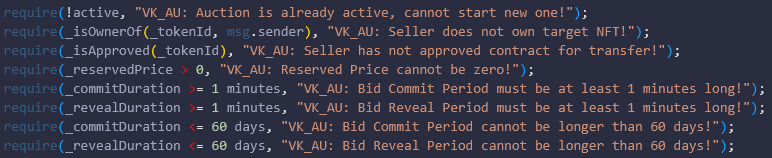
\includegraphics[width=1.0\linewidth]{../Images/startAuctionRequires.png}
        \caption{Code Snippet of input validation in startAuction function}
    \end{figure}
    \item \textbf{Commit-Reveal:} Correctly implemented using \texttt{\detokenize{EfficientHashLib.hash}} including bidder address, amount, nonce, token ID, and auction ID, preventing hash collisions across different contexts. Reveal logic correctly compares recomputed hash with stored \texttt{\detokenize{bidHash}}.
    \begin{figure}[H]
        \centering
        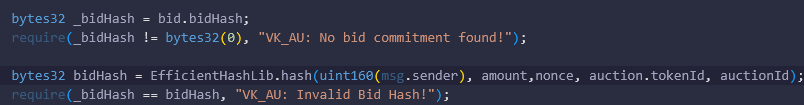
\includegraphics[width=1.0\linewidth]{../Images/hashCheck.png}
        \caption{Code Snippet of Hash check}
    \end{figure}
    \item \textbf{Access Control:} NFT ownership/approval checked in \texttt{\detokenize{startAuction}}. \texttt{\detokenize{commitBid}} prevents the seller bidding (\texttt{\detokenize{require(msg.sender != auction.seller, ...)}}). Phase timing is enforced.
    \item \textbf{Safe ETH Transfer:} Uses Solady's \texttt{\detokenize{SafeTransferLib}} (\texttt{\detokenize{safeTransferETH}}) for transfers in \texttt{\detokenize{endAuction}} and \texttt{\detokenize{withdraw}}, reducing risks associated with raw calls or \texttt{\detokenize{.transfer()}}.
\end{itemize}

\textbf{Efficiency:}
\begin{itemize}
    \item \textbf{Struct Packing:} Good use of smaller types (\texttt{\detokenize{uint128}}, \texttt{\detokenize{uint32}}, \texttt{\detokenize{uint8}}, \texttt{\detokenize{bool}}) aims to reduce storage costs. \texttt{\detokenize{CommittedBid}} fits in 2 slots. \texttt{\detokenize{Auction}} fits in 5 slots.
    \begin{figure}[H]
        \centering
        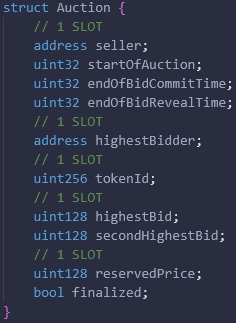
\includegraphics[]{../Images/structAuction.png}
        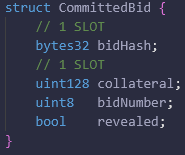
\includegraphics[]{../Images/structBid.png}
        \caption{Code Snippet of struct CommitedBid and Auction}
    \end{figure}
    \item \textbf{Hashing Library:} \texttt{\detokenize{EfficientHashLib}} potentially saves gas over standard hashing.
    \item \textbf{Auctions Array:} Using \texttt{\detokenize{Auction[] public auctions;}} and incrementing \texttt{\detokenize{auctionId}} only when ending an auction means only the latest auction is directly accessible via \texttt{\detokenize{auctions[auctionId]} during its active phase}. Accessing past auctions requires iterating or knowing the specific index. \texttt{\detokenize{auctions.push()}} gas cost increases over time. Managing only one active auction simplifies state but differs from typical multi-auction platforms. Use of \texttt{\detokenize{delete committedBids[_auctionId][msg.sender];}} reclaims some gas upon withdrawal.
    \begin{figure}[H]
        \centering
        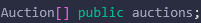
\includegraphics[width=1.0\linewidth]{../Images/auctionArray.png}
        \caption{Code Snippet of Auction[] public auctions Array}
    \end{figure}
\end{itemize}

\textbf{Fairness:}
\begin{itemize}
    \item \textbf{Gas Costs in \texttt{\detokenize{endAuction}} (Push Pattern):} The caller of \texttt{\detokenize{endAuction}} bears gas costs for ETH transfers to the seller and potentially the winner (refund), plus the NFT transfer. This contrasts with a pull pattern and can disincentivise calling the function, potentially delaying settlement.
    \begin{figure}[H]
        \centering
        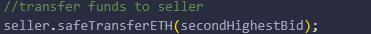
\includegraphics[width=1.0\linewidth]{../Images/safeTransferETH.png}
        \caption{Code Snippet of safeTransferETH in end Auction}
    \end{figure}
    \item \textbf{Multiple Commits:} Allows up to 3 commits (\texttt{\detokenize{bid.bidNumber < 3}}). Collateral is cumulative (\texttt{\detokenize{bid.collateral += uint128(msg.value);}}), but only the last hash (\texttt{\detokenize{bid.bidHash = bidHash;}}) matters for reveal. This might allow tactical deposit increases but primarily seems to add complexity and potential gas usage without clear benefit over a single commit model. It doesn't seem inherently unfair.
    \begin{figure}[H]
        \centering
        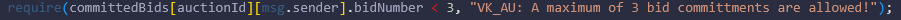
\includegraphics[width=1.0\linewidth]{../Images/multipleCommit.png}
        \caption{Code Snippet of maximum of 3 commits logic}
    \end{figure}
    \item \textbf{Tie-breaking (Reveal Time):} Logic \texttt{\detokenize{if(amount > auction.highestBid)}} implies the first reveal wins ties for the highest bid, as subsequent equal bids won't overwrite \texttt{{auction. \newline highestBidder}}. This differs from using commit time but is still deterministic.
    \begin{figure}[H]
        \centering
        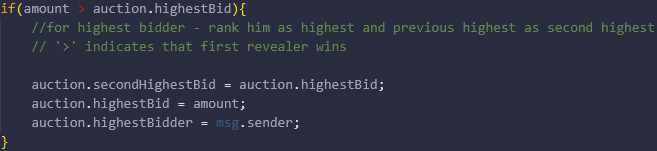
\includegraphics[width=1.0\linewidth]{../Images/revealTime.png}
        \caption{Code Snippet of reveal time tie breaking}
    \end{figure}
    \item \textbf{Withdrawal Gas:} Losers and the winner (for refund difference handled in \texttt{\detokenize{endAuction}}) call \texttt{\detokenize{withdraw}} paying their own gas, which is fair.
\end{itemize}

\subsection{Vulnerabilities Discovered}
No critical security flaws were found. Areas for consideration:
\begin{itemize}
    \item \textbf{Gas Burden / Potential Delay for \texttt{\detokenize{endAuction}}:} The push payments within \texttt{\newline {endAuction}} create a variable and potentially high gas cost for the caller, which could lead to delays if no party is incentivised to trigger it promptly. This is more a design choice trade-off than a vulnerability allowing theft.
    \item \textbf{Complexity of Multiple Commits:} Allowing multiple commits increases the contract's state size (\texttt{\detokenize{bidNumber}}) and logic (\texttt{\detokenize{require(..., bidNumber < 3}})), adding slight gas overhead and complexity without a clear strategic advantage for bidders (since only the last hash counts). It could potentially be used for minor griefing.
    \item \textbf{Auction Array Growth:} The unbounded \texttt{\detokenize{auctions.push()}} could eventually lead to very high gas costs for starting new auctions, though this requires a huge number of auctions to become problematic.
\end{itemize}

\newpage
\section{Contract Addresses and Transaction Hashes}
\subsection{Contract Address}
My Sepolia Contract Address: [0xbCabCa54D6d26c19AFe4078C6e20eaFfd8B1716b]

\subsection{Interaction Transaction Hashes}
Interaction for Address(My contract): \newline [0xbCabCa54D6d26c19AFe4078C6e20eaFfd8B1716b]
\begin{table}[H]
  \centering
  \begin{tabularx}{\linewidth}{l l >{\raggedright\arraybackslash}X}
    \toprule
    Actor             & Action                                  & Transaction Hash \\
    \midrule
    Me                & \texttt{\detokenize{startAuction}}      & \seqsplit{0x660d17ae5157ad213c9b38a2b485a4e8e6a594b2b6c2f6987c30a7aea34dcc0a} \\
    Me (Failed)       & \texttt{\detokenize{commitBid}}         & \seqsplit{0xadd6a9d9f9ca2afcf2de0c8bfb6acde52b8ef0557e1c18cd6225391c167601f1}\\
    Fellow Student    & \texttt{\detokenize{commitBid}}         & \seqsplit{0xbd8d51ef0d60c66a2e4d9b44d4b5050a1a56c7e0d126bc95e167d0f0b941ccfe} \\
    Fellow Student    & \texttt{\detokenize{revealBid}}         & \seqsplit{0x6a757b155b1cb4a5127c17659496b71c544cca1e4e248b860a9d4d902e64d958} \\
    Fellow Student    & \texttt{\detokenize{finalisedAuction}} & \seqsplit{0x44bdfd51a198a071442366cfff4dfed5bf884a417793f47e0ab96e27c217aeed} \\
    Fellow Student    & \texttt{\detokenize{withdrawFunds}}    & \seqsplit{0x4139420cc6402a37095417f8f58c103d21a7a5086e6b39e9c585bb54a9831f5d} \\
    \bottomrule
  \end{tabularx}
\end{table}
Interaction for Address(Fellow Student's contract): \newline [0xC8269b326055480513cB655a03d22963e4D342f4]
\begin{table}[H]
  \centering
  \begin{tabularx}{\linewidth}{l l >{\raggedright\arraybackslash}X}
    \toprule
    Actor             & Action                                  & Transaction Hash \\
    \midrule
    Fellow Student    & \texttt{\detokenize{startAuction}}      & \seqsplit{0x18bc588de6caa8751f03206e75c6005f04358f532f6e7c28f90f4c6371e155d1} \\
    Me                & \texttt{\detokenize{commitBid}}         & \seqsplit{0xa6e7336d7a01e54ac826367186b0673c0a7056aea5e432a4eebd615e0d12eeb4} \\
    Fellow Student    & \texttt{\detokenize{commitBid}}         & \seqsplit{0xf721195c9f18d243c2bd05e29a70fac35af9c93dc0ab19bfec5db20c5ad216d4} \\
    Me                & \texttt{\detokenize{revealBid}}         & \seqsplit{0x0ec506c83bcf8338de3df838fad7996eec4b130a4003cc7d588f48cc6e825ef0} \\
    Fellow Student    & \texttt{\detokenize{revealBid}}         & \seqsplit{0x04e4f7030cc54bcbee8135728a7f3686edc4763f35781f42f770ff4eea245dc2} \\
    Me                & \texttt{\detokenize{endAuction}}        & \seqsplit{0x13359bf9634f50c2890786d5566f0e5dd0fb9021f20fde0e9837b3d2c7dcb792} \\
    Me                & \texttt{\detokenize{withdraw}}          & \seqsplit{0xf51694fea8b36e17d8d35725b3dd8c36fc192c5d0cd6eecc2daa7478d5f05276} \\
    Fellow Student    & \texttt{\detokenize{withdraw}}          & \seqsplit{0xf2b1d005abed83cb4bfc1746cd664965f9187251e5af94a433743fe6fb1a56c7} \\
    \bottomrule
  \end{tabularx}
\end{table}

\newpage
\section{Contract Code}
% --- EXAMPLE PLACEHOLDER FOR CODE ---
\begin{lstlisting}
/// SPDX-License-Identifier: MIT
pragma solidity ^0.8.0;

// Imports the standard interface for an ERC721 NFT.
import "@openzeppelin/contracts/token/ERC721/IERC721.sol";

// Imports the interface required for the contract to safely receive an NFT.
import "@openzeppelin/contracts/token/ERC721/IERC721Receiver.sol";

// This contract implements the receiver interface, allowing it to hold an NFT during the auction.
contract VickreyAuction is IERC721Receiver {

    // State Variables
    // Stores the address of the ClassNFT contract. It's set once and unchangeable.
    IERC721 public immutable nftContract;

    // A custom data structure to hold all information about a single auction.
    struct Auction{
        address payable seller;         // The person selling the NFT.
        uint256 nftTokenId;             // The unique ID of the NFT being sold.
        uint256 reservePrice;           // The minimum price the seller will accept.
        uint256 biddingEndTime;         // The timestamp when the commit/bidding phase ends.
        uint256 revealEndTime;          // The timestamp when the reveal phase ends.
        bool isActive;                    // The flag to check activity of the auction.
        bool isFinalised;                 // The flag to check whether auction has been finalised.
        address payable highestBidder;  // The current winning bidder.
        uint256 highestBid;             // The highest bid amount revealed so far.
        uint256 secondHighestBid;       // The second-highest bid amount revealed.
        uint256 highestBidCommitBlock;  // The block number of the highest bid, used for tie-breaking.
    }

    // A custom data structure to hold a bidder's information for an auction.
    struct Bid{
        bytes32 commitment;            // The user's hashed bid (keccak256(amount, nonce)).
        uint256 deposit;               // The total Wei the bidder locked up with their bid.
        uint256 commitBlock;           // The block number when the bid was committed.
        bool isRevealed;                 // The flag to check whether bid was revealed.
    }

    // A counter to give each new auction a unique ID. Not using counters library since version ^0.8 prevents underflow/overflow
    uint256 public auctionCounter;

    // Mappings
    // A mapping from an auction's ID to its Auction data.
    mapping(uint256 => Auction) public auctions;

    // A nested mapping from an auction ID to bidder's address to bidder's Bid data.
    mapping(uint256 => mapping(address => Bid)) public bids;

    // A mapping to track how much Wei each address is owed from auctions.
    // This is for the "pull" withdrawal pattern, which is more secure.
    mapping(address => uint256) public pendingWithdrawals;

    // Events
    // Logs the creation and key details of a new auction.
    event AuctionStarted(
        uint256 indexed auctionId,
        address indexed seller,
        uint256 indexed nftTokenId,
        uint256 reservePrice,
        uint256 biddingEndTime,
        uint256 revealEndTime
    );

    // Logs that a bidder has submitted their hidden (committed) bid.
    event BidCommitted(
        uint256 indexed auctionId,
        address indexed bidder,
        bytes32 commitment
    );

    // Logs that a bidder has successfully revealed their bid amount.
    event BidRevealed(
        uint256 indexed auctionId,
        address indexed bidder,
        uint256 amount
    );

    // Logs the final outcome of an auction, including the winner and final price.
    event AuctionFinalised(
        uint256 indexed auctionId,
        address winner,
        uint256 paymentAmount
    );

    // Logs a successful withdrawal of funds by a specific user.
    event FundsWithdrawn(
        address indexed user,
        uint256 amount
    );

    // Functions
    // The constructor runs once when the contract is deployed.
    // It permanently sets the address of the ClassNFT contract.
    constructor(address _nftContract) {
        // Pass the address of ClassNFT.sol (0x1546Bd67237122754D3F0CB761c139f81388b210)
        require(_nftContract != address(0), "Invalid NFT contract address.");
        nftContract = IERC721(_nftContract);
    }

    // This function is required by IERC721Receiver. It allows the contract
    // to accept an NFT from the safeTransferFrom function.
    function onERC721Received(
        address operator,
        address from,
        uint256 tokenId,
        bytes calldata data
    ) external override returns (bytes4) {
        return this.onERC721Received.selector;
    }

    // Creates a new auction.
    function startAuction(
        uint256 _tokenId,          // The ID of the NFT to be auctioned off.
        uint256 _reservePrice,     // The minimum price.
        uint256 _biddingDuration,  // How long the bidding phase lasts (seconds).
        uint256 _revealDuration    // How long the reveal phase lasts (seconds).
    ) external {
        // Checks that the person starting the auction is the real owner of the NFT.
        require(nftContract.ownerOf(_tokenId) == msg.sender, "Not the NFT's owner.");
        require(_biddingDuration > 0, "Bidding duration must be more than 0.");
        require(_revealDuration > 0, "Reveal duration must be more than 0.");

        // Checks that the contract is approved to take the NFT.
        require( nftContract.getApproved(_tokenId) == address(this) 
            || nftContract.isApprovedForAll(msg.sender, address(this)),
            "Contract not approved for this NFT."
        );

        // Transfers the NFT from the seller into this contract, which acts as a secure escrow.
        nftContract.safeTransferFrom(msg.sender, address(this), _tokenId);

        // Sets up the new auction's data in storage.
        uint256 auctionId = auctionCounter;
        Auction storage newAuction = auctions[auctionId];

        newAuction.seller = payable(msg.sender);
        newAuction.nftTokenId = _tokenId;
        newAuction.reservePrice = _reservePrice;
        newAuction.biddingEndTime = block.timestamp + _biddingDuration;
        newAuction.revealEndTime = newAuction.biddingEndTime + _revealDuration;
        newAuction.isActive = true;
        newAuction.isFinalised = false;

        // Increments the counter so the next auction gets a new ID.
        auctionCounter++;

        emit AuctionStarted(
            auctionId, 
            newAuction.seller, 
            newAuction.nftTokenId, 
            newAuction.reservePrice, 
            newAuction.biddingEndTime, 
            newAuction.revealEndTime
        );
    }

    // Allows a bidder to commit their hashed bid and deposit.
    function commitBid(
        uint256 _auctionId,  // The ID of the auction to bid on.
        bytes32 _commitment  // The hashed bid (keccak256(amount, nonce)).
    ) external payable {
        Auction storage auction = auctions[_auctionId];

        // Checks to ensure the auction is in a valid state for bidding.
        require(msg.sender != auction.seller, "Seller cannot bid.");
        require(auction.isActive, "Auction not active.");
        require(block.timestamp < auction.biddingEndTime, "Bidding phase over.");

        // Check to ensure a bidder can only commit once.
        require(bids[_auctionId][msg.sender].commitment == bytes32(0), "Bid has already been committed.");

        require(msg.value > 0, "Deposit must be more than 0");
        require(_commitment != bytes32(0), "Commitment cannot be zero");

        // Stores the bidder's information.
        Bid storage newBid = bids[_auctionId][msg.sender];
        newBid.commitment = _commitment;
        newBid.deposit = msg.value;         // msg.value is the amount of Wei sent.
        newBid.commitBlock = block.number;  // Stores the block number for tie-breaking.
        newBid.isRevealed = false;

        emit BidCommitted(_auctionId, msg.sender, newBid.commitment);
    }

    // Allows a bidder to reveal their actual bid amount and nonce.
    function revealBid(
        uint256 _auctionId,  // The auction ID.
        uint256 _bidAmount,  // The real bid amount.
        bytes32 _nonce       // The secret random string.
    ) external {
        Auction storage auction = auctions[_auctionId];
        Bid storage bid = bids[_auctionId][msg.sender];

        // Checks to ensure the auction is in the correct reveal phase.
        require(auction.isActive, "Auction not active.");
        require(block.timestamp > auction.biddingEndTime, "Bidding phase not over.");
        require(block.timestamp < auction.revealEndTime, "Reveal phase over.");

        // Checks that the bidder has a committed bid to reveal.
        require(bid.commitment != 0, "No bid committed");
        require(!bid.isRevealed, "Bid already revealed");

        // Recalculate and check the hash to see if it matches the one committed earlier.
        bytes32 commitment = keccak256(abi.encodePacked(_bidAmount, _nonce));
        require(bid.commitment == commitment, "Invalid reveal");

        // Check if the revealed amount is covered by their deposit.
        require(bid.deposit >= _bidAmount, "Deposit less than required amount");

        // Marks the bid as revealed to prevent revealing again.
        bid.isRevealed = true;

        // Check if bid meet reserve price threshold.
        if(_bidAmount < auction.reservePrice){
            emit BidRevealed(_auctionId, msg.sender, _bidAmount);
            return; //Exit the function early
        }

        // Winner Determination Logic
        // If current bid is the new highest
        if(_bidAmount > auction.highestBid) {
            // The old highest bid becomes the new second-highest.
            auction.secondHighestBid = auction.highestBid;
            // This bid becomes the new highest.
            auction.highestBid = _bidAmount;
            auction.highestBidder = payable(msg.sender);
            auction.highestBidCommitBlock = bid.commitBlock;

        // If this bid is tied with the current highest
        } else if (_bidAmount == auction.highestBid) {

            // TIE-BREAKING RULE: Check if this bid was committed in an earlier block.
            if (bid.commitBlock < auction.highestBidCommitBlock) {
                // Current bid wins the tie breaking
                auction.secondHighestBid = auction.highestBid; // The tied amount is now second-highest.
                auction.highestBidder = payable(msg.sender);
                auction.highestBidCommitBlock = bid.commitBlock;
            } else {
                //Old bid comes first, the current bid is now second highest
                auction.secondHighestBid = _bidAmount;
            }
        // If current bid is not the highest, but is higher than the current second-highest
        } else if (_bidAmount > auction.secondHighestBid) {
            // Current bid becomes the new second-highest bid.
            auction.secondHighestBid = _bidAmount;
        }

        emit BidRevealed(_auctionId, msg.sender, _bidAmount);
    }

    // Finalises the auction, calculates the winner and price, and handles refunds.
    function finalisedAuction(
        uint256 _auctionId  // The auction ID to end.
    ) external {
        Auction storage auction = auctions[_auctionId];

        // Checks to ensure the auction can be finalised.
        require(auction.isActive, "Auction not active.");
        require(block.timestamp > auction.revealEndTime, "Reveal phase not over.");
        require(!auction.isFinalised, "Auction already finalised");

        // Marks the auction as finished so this can't be run again.
        auction.isFinalised = true;
        auction.isActive = false;

        address payable winner = auction.highestBidder;
        uint256 paymentAmount = 0;

        // Check if there was a winner, at least one valid bid above reserve.
        if (winner != address(0)){

            // Second-Price Logic
            if (auction.secondHighestBid == 0) {
                // If only one bid, the winner pays the reserve price.
                paymentAmount = auction.reservePrice;
            } else {
                 // If multiple bids, winner pays  the max between second-highest and reserve price.
                paymentAmount = (auction.secondHighestBid > auction.reservePrice) ? auction.secondHighestBid : auction.reservePrice;
            }

            // Credit the seller's internal account. They can withdraw this later.
            pendingWithdrawals[auction.seller] += paymentAmount;

            // Calculate the winner's refund (Deposit - Price Paid).
            uint256 winnerDeposit = bids[_auctionId][winner].deposit;
            uint256 winnerRefund = winnerDeposit - paymentAmount;

            // If the winner is owed a refund, credit their internal account.
            if (winnerRefund > 0){
                pendingWithdrawals[winner] += winnerRefund;
            }
        }

        emit AuctionFinalised(_auctionId, winner, paymentAmount); 

        // NFT Transfer
         // If there's a winner, send them the NFT.
        if (winner != address(0)) {
            nftContract.safeTransferFrom(
                address(this),
                winner,
                auction.nftTokenId
            );
        
        // If no winner, return the NFT to the seller.
        } else {
            nftContract.safeTransferFrom(
                address(this),
                auction.seller,
                auction.nftTokenId
            );
        }        
    }

    // Allows losing bidders to make their deposits claimable by transferring their deposits to withdrawable balance.
    function claimLosingBid(
        uint256 _auctionId  // The auction they bid in.
    ) external {
        Auction storage auction = auctions[_auctionId];

        // Checks that the auction is over and the caller is not the winner.
        require(auction.isFinalised, "Auction not finalised");
        require(msg.sender != auction.highestBidder, "Winner cannot claim refund here");

        Bid storage bid = bids[_auctionId][msg.sender];
        uint256 amount = bid.deposit;

        require(amount > 0, "No deposit to claim");

        // Set deposit to 0 before adding to withdrawal list.
        // This prevents a re-entrancy attack where they could claim multiple times.
        bid.deposit = 0;

        // Credit the bidder's internal account.
        pendingWithdrawals[msg.sender] += amount;
    }

    // Allows any user to withdraw their balance from the contract.
    // This is the "pull" part of the secure pull-over-push pattern.
    function withdrawFunds() external{
        // Get the amount this user is owed.
        uint256 amount = pendingWithdrawals[msg.sender];

        require(amount > 0, "No funds to withdraw");

        // Set their internal balance to 0 before sending the Wei.
        // This is the most critical part of preventing re-entrancy attacks.
        pendingWithdrawals[msg.sender] = 0;

        // Send the Wei to the user.
        (bool success, ) = msg.sender.call{value: amount}("");
        require(success, "Transfer failed");

        emit FundsWithdrawn(msg.sender, amount);
    }
}
\end{lstlisting}


% --- DOCUMENT END ---
\end{document}

